\documentclass[aspectratio=169,10pt]{ctexbeamer}

\usetheme{Madrid}
\usecolortheme{default}

\usepackage{amsmath,amssymb,mathtools,bm}
\usepackage{tikz}
\usetikzlibrary{arrows.meta,calc,positioning}

\makeatletter
\def\input@path{{../模板/}}
\makeatother
\usepackage{yingxing-beamer}

\definecolor{MainBlue}{RGB}{25,70,140}
\definecolor{AccentRed}{RGB}{180,60,45}
\definecolor{SoftBg}{RGB}{246,248,252}
\setbeamercolor{alerted text}{fg=AccentRed}

\newcommand{\R}{\mathbb{R}}
\newcommand{\dd}{\,\mathrm{d}}
\newcommand{\ee}{\mathrm{e}}
\newcommand{\ii}{\mathrm{i}}

\title{微分中值定理}
\subtitle{}
\author{}
\date{}

\begin{document}

\begin{frame}
  \titlepage
\end{frame}

\begin{frame}{本次内容}
\small
\tableofcontents
\end{frame}

\section{核心定理}

\begin{frame}[t]{基本思想}
\small
\begin{block}{变化量与变化率}
微分中值定理把函数值的差
\[
  f(b)-f(a)
\]
和区间内部某点的导数
\[
  f'(\xi)
\]
联系起来。
\end{block}

\begin{block}{证明策略}
三个主要定理都可归结为同一个想法：构造辅助函数，使端点函数值相等，然后使用 Rolle 定理。
\end{block}
\end{frame}

\begin{frame}[t]{定理 1：Rolle 定理}
\small
\begin{block}{结论}
设 $f$ 在 $[a,b]$ 上连续，在 $(a,b)$ 中可微，且
\[
  f(a)=f(b).
\]
则存在 $\xi\in(a,b)$，使得
\[
  f'(\xi)=0.
\]
\end{block}

\begin{block}{证明}
连续函数在闭区间上取到最大值 $M$ 与最小值 $m$。
若 $M=m$，则 $f$ 为常值函数，结论显然成立。
若 $M>m$，由于 $f(a)=f(b)$，最大值或最小值至少有一个在内点 $\xi$ 处取得。
由 Fermat 定理，
\[
  f'(\xi)=0.
\]
\end{block}
\end{frame}

\begin{frame}[t,shrink=5]{定理 2：Lagrange 中值定理}
\small
\begin{block}{结论}
设 $f$ 在 $[a,b]$ 上连续，在 $(a,b)$ 中可微，则存在 $\xi\in(a,b)$，使得
\[
  f'(\xi)=\frac{f(b)-f(a)}{b-a}.
\]
等价地，
\[
  f(b)-f(a)=f'(\xi)(b-a).
\]
\end{block}

\begin{block}{证明}
令
\[
  F(x)=f(x)-\left[f(a)+\frac{f(b)-f(a)}{b-a}(x-a)\right].
\]
则 $F(a)=F(b)=0$。由 Rolle 定理，存在 $\xi\in(a,b)$，使得 $F'(\xi)=0$，即
\[
  f'(\xi)=\frac{f(b)-f(a)}{b-a}.
\]
\end{block}
\end{frame}

\begin{frame}[t]{Rolle 与 Lagrange 的几何图像}
\small
\begin{columns}[T,onlytextwidth]
\begin{column}{0.48\textwidth}
\begin{center}
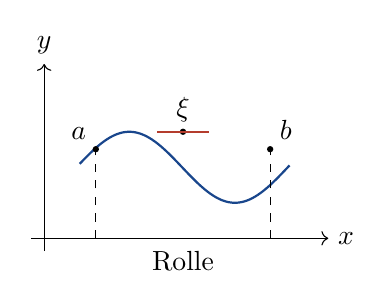
\begin{tikzpicture}[scale=0.82]
\draw[->] (-0.2,0)--(4.4,0) node[right] {$x$};
\draw[->] (0,-0.2)--(0,2.7) node[above] {$y$};
\draw[thick,MainBlue,domain=0.55:3.8,smooth,samples=80]
  plot(\x,{1.1+0.55*sin(110*(\x-0.5))});
\draw[dashed] (0.8,0)--(0.8,1.38);
\draw[dashed] (3.5,0)--(3.5,1.38);
\fill (0.8,1.38) circle (1.4pt) node[above left] {$a$};
\fill (3.5,1.38) circle (1.4pt) node[above right] {$b$};
\fill (2.15,1.65) circle (1.4pt) node[above] {$\xi$};
\draw[AccentRed,thick] (1.75,1.65)--(2.55,1.65);
\node at (2.15,-0.35) {Rolle};
\end{tikzpicture}
\end{center}
\end{column}
\begin{column}{0.48\textwidth}
\begin{center}
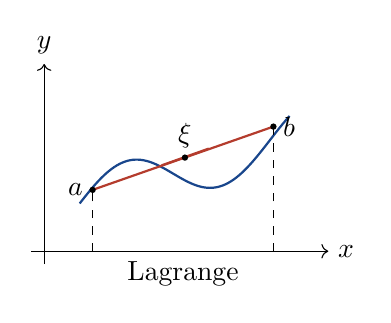
\begin{tikzpicture}[scale=0.82]
\draw[->] (-0.2,0)--(4.4,0) node[right] {$x$};
\draw[->] (0,-0.2)--(0,2.9) node[above] {$y$};
\draw[thick,MainBlue,domain=0.55:3.8,smooth,samples=80]
  plot(\x,{0.5+0.35*\x+0.45*sin(120*(\x-0.5))});
\draw[AccentRed,thick] (0.75,0.95)--(3.55,1.93);
\draw[dashed] (0.75,0)--(0.75,0.95);
\draw[dashed] (3.55,0)--(3.55,1.93);
\fill (0.75,0.95) circle (1.4pt) node[left] {$a$};
\fill (3.55,1.93) circle (1.4pt) node[right] {$b$};
\draw[AccentRed,thick] (1.82,1.33)--(2.55,1.59);
\fill (2.18,1.45) circle (1.4pt) node[above] {$\xi$};
\node at (2.15,-0.35) {Lagrange};
\end{tikzpicture}
\end{center}
\end{column}
\end{columns}
\end{frame}

\begin{frame}[t]{Lagrange 定理的解释}
\small
\begin{block}{物理解释}
如果 $f(x)$ 表示位置，则
\[
  \frac{f(b)-f(a)}{b-a}
\]
表示从 $a$ 到 $b$ 的平均速度。Lagrange 定理说明：某个时刻 $\xi$ 的瞬时速度等于这段时间的平均速度。
\end{block}

\begin{block}{几何解释}
令
\[
  \ell(x)=f(a)+\frac{f(b)-f(a)}{b-a}(x-a).
\]
这是连接 $(a,f(a))$ 与 $(b,f(b))$ 的割线。令 $F(x)=f(x)-\ell(x)$，则 $F(a)=F(b)=0$，问题化为 Rolle 定理。
\end{block}
\end{frame}

\begin{frame}[t]{定理 3：Cauchy 中值定理}
\small
\begin{block}{结论}
设 $f,g$ 在 $[a,b]$ 上连续，在 $(a,b)$ 中可微，且
\[
  g'(x)\ne0,\qquad x\in(a,b).
\]
则存在 $\xi\in(a,b)$，使得
\[
  \frac{f(b)-f(a)}{g(b)-g(a)}
  =
  \frac{f'(\xi)}{g'(\xi)}.
\]
\end{block}

\begin{block}{证明}
由 Rolle 定理可知 $g(b)\ne g(a)$。令
\[
  F(x)=f(x)-\left[f(a)+\frac{f(b)-f(a)}{g(b)-g(a)}(g(x)-g(a))\right].
\]
则 $F(a)=F(b)=0$，由 Rolle 定理可得结论。
\end{block}
\end{frame}

\begin{frame}[t]{三个中值定理的关系}
\footnotesize
\begin{block}{包含关系}
\[
\begin{array}{ccl}
\text{Cauchy 定理} & \xrightarrow{\ g(x)=x\ } & \text{Lagrange 定理}\\[0.4em]
\text{Lagrange 定理}+f(a)=f(b) & \Longrightarrow & \text{Rolle 定理}
\end{array}
\]
\end{block}

\begin{block}{对应公式}
\[
  \frac{f(b)-f(a)}{g(b)-g(a)}
  =
  \frac{f'(\xi)}{g'(\xi)}
  \quad\Longrightarrow\quad
  \frac{f(b)-f(a)}{b-a}=f'(\xi).
\]
若 $f(a)=f(b)$，则进一步得到 $f'(\xi)=0$。
\end{block}
\end{frame}

\section{典型应用}

\begin{frame}[t]{例 1：正弦函数的 Lipschitz 性}
\small
证明
\[
  |\sin x-\sin y|\le |x-y|,\qquad \forall x,y\in\R.
\]

由 Lagrange 中值定理，存在 $\xi$ 介于 $x,y$ 之间，使得
\[
  \sin x-\sin y=\cos\xi\,(x-y).
\]
因此
\[
  |\sin x-\sin y|
  =|\cos\xi|\,|x-y|
  \le |x-y|.
\]

\begin{alertblock}{推广}
若 $f'$ 有界，即 $|f'|\le M$，则
\[
  |f(x)-f(y)|\le M|x-y|.
\]
\end{alertblock}
\end{frame}

\begin{frame}[t]{例 2：构造辅助函数}
\small
设 $f$ 在 $[a,b]$ 上连续，在 $(a,b)$ 中可导，且
\[
  f(a)=f(b)=0.
\]
证明存在 $\xi\in(a,b)$，使
\[
  f'(\xi)+f(\xi)=0.
\]

令
\[
  g(x)=\ee^x f(x).
\]
则
\[
  g(a)=g(b)=0.
\]
由 Rolle 定理，存在 $\xi\in(a,b)$，使得 $g'(\xi)=0$。又
\[
  g'(x)=\ee^x f(x)+\ee^x f'(x)=\ee^x\bigl(f'(x)+f(x)\bigr),
\]
且 $\ee^\xi>0$，故 $f'(\xi)+f(\xi)=0$。
\end{frame}

\begin{frame}[t]{例 3：指数函数不等式}
\small
证明
\[
  \ee^x\ge 1+x,\qquad x\in\R,
\]
且等号仅当 $x=0$ 时成立。

令
\[
  f(x)=\ee^x-(1+x).
\]
显然 $f(0)=0$。当 $x\ne0$ 时，由 Lagrange 中值定理，存在 $\xi$ 介于 $0,x$ 之间，使得
\[
  f(x)-f(0)=f'(\xi)x=(\ee^\xi-1)x.
\]
若 $x>0$，则 $\xi>0$，故 $\ee^\xi-1>0$；若 $x<0$，则 $\xi<0$，故 $\ee^\xi-1<0$。
两种情形均有
\[
  f(x)>0.
\]
\end{frame}

\begin{frame}[t]{例 4：二阶中值形式}
\small
设 $f$ 在 $[a,b]$ 上连续，在 $(a,b)$ 中二阶可导，且
\[
  f(a)=f(b)=0.
\]
证明：对任意 $c\in[a,b]$，存在 $\xi\in(a,b)$，使
\[
  f(c)=\frac{f''(\xi)}2(c-a)(c-b).
\]
\end{frame}

\begin{frame}[t]{例 4：证明}
\small
若 $c=a$ 或 $c=b$，结论显然。设 $c\in(a,b)$，令
\[
  F(x)=f(x)-\frac{f(c)}{(c-a)(c-b)}(x-a)(x-b).
\]
则
\[
  F(a)=F(c)=F(b)=0.
\]
由 Rolle 定理，存在
\[
  \xi_1\in(a,c),\qquad \xi_2\in(c,b),
\]
使得
\[
  F'(\xi_1)=F'(\xi_2)=0.
\]
再对 $F'$ 使用 Rolle 定理，存在 $\xi\in(\xi_1,\xi_2)$，使得 $F''(\xi)=0$。
而
\[
  F''(x)=f''(x)-\frac{2f(c)}{(c-a)(c-b)}.
\]
代入 $x=\xi$ 即得结论。
\end{frame}

\begin{frame}[t,shrink=5]{推广：多个零点}
\footnotesize
设 $f$ 是 $n$ 阶可导函数，且 $f(x)=0$ 有 $n$ 个不同的解
\[
  x_1,x_2,\ldots,x_n.
\]
则对任意 $c$，存在 $\xi$，使得
\[
  f(c)=\frac1{n!}f^{(n)}(\xi)\prod_{i=1}^n(c-x_i).
\]

\begin{block}{证明主线}
令
\[
  F(x)=f(x)-\frac{f(c)}{\prod_{i=1}^n(c-x_i)}
  \prod_{i=1}^n(x-x_i).
\]
则 $F$ 有 $n+1$ 个不同零点。对 $F$ 反复使用 Rolle 定理，可得存在 $\xi$ 使
\[
  F^{(n)}(\xi)=0.
\]
再利用
\[
  \left(\prod_{i=1}^n(x-x_i)\right)^{(n)}=n!
\]
即可得到公式。
\end{block}
\end{frame}

\begin{frame}[t]{Lagrange 插值多项式及余项}
\footnotesize
设 $f$ 为 $n$ 阶可导函数，$x_1,\ldots,x_n$ 为互异节点。定义
\[
  p_{n-1}(x)=
  \sum_{i=1}^n
  f(x_i)\prod_{j\ne i}\frac{x-x_j}{x_i-x_j}.
\]
则 $p_{n-1}$ 的次数不超过 $n-1$，且
\[
  p_{n-1}(x_i)=f(x_i),\qquad i=1,\ldots,n.
\]

由于 $f-p_{n-1}$ 有 $n$ 个不同零点，由上一页公式可得
\[
  f(x)-p_{n-1}(x)
  =
  \frac1{n!}f^{(n)}(\xi)\prod_{i=1}^n(x-x_i).
\]
\end{frame}

\begin{frame}[t]{例 5：Legendre 多项式的实根}
\small
\begin{block}{题目}
证明
\[
  \frac{\dd^n}{\dd x^n}(x^2-1)^n
\]
在 $(-1,1)$ 中有 $n$ 个不同实根，其中 $n\ge1$。
\end{block}

\begin{block}{证明主线}
多项式 $(x^2-1)^n$ 在 $x=-1$ 与 $x=1$ 处有 $n$ 重零点。
反复使用 Rolle 定理：每求一次导数，端点处零点的重数下降一阶，同时区间内部增加由 Rolle 定理保证的零点。
经过 $n$ 次求导后，
\[
  \frac{\dd^n}{\dd x^n}(x^2-1)^n
\]
在 $(-1,1)$ 中至少有 $n$ 个不同零点。由于它是 $n$ 次多项式，故恰有 $n$ 个不同实根。
\end{block}
\end{frame}

\section{课后习题与解答}

\begin{frame}[t]{习题 1：题目}
\small
证明多项式
\[
  x^3-3x+c
\]
在 $[0,1]$ 上不存在两个不同的实根。
\end{frame}

\begin{frame}[t]{习题 1：解答}
\small
设
\[
  f(x)=x^3-3x+c.
\]
若它在 $[0,1]$ 上有两个不同实根 $\alpha<\beta$，则
\[
  f(\alpha)=f(\beta)=0.
\]
由 Rolle 定理，存在 $\xi\in(\alpha,\beta)\subset(0,1)$，使得
\[
  f'(\xi)=0.
\]
但
\[
  f'(x)=3x^2-3=3(x^2-1)<0,\qquad 0<x<1,
\]
不可能等于 $0$。矛盾。因此该多项式在 $[0,1]$ 上不存在两个不同实根。
\end{frame}

\begin{frame}[t]{习题 2：题目}
\small
设 $f$ 在 $[a,b]$ 上连续，在 $(a,b)$ 中可微，且
\[
  f(a)=f(b)=0.
\]
证明存在 $\xi\in(a,b)$，使得
\[
  f'(\xi)=2f(\xi).
\]
\end{frame}

\begin{frame}[t]{习题 2：解答}
\small
构造
\[
  g(x)=\ee^{-2x}f(x).
\]
则 $g$ 在 $[a,b]$ 上连续，在 $(a,b)$ 中可微，并且
\[
  g(a)=g(b)=0.
\]
由 Rolle 定理，存在 $\xi\in(a,b)$，使
\[
  g'(\xi)=0.
\]
而
\[
  g'(x)=\ee^{-2x}\bigl(f'(x)-2f(x)\bigr).
\]
由于 $\ee^{-2\xi}\ne0$，得到
\[
  f'(\xi)-2f(\xi)=0,
\]
即
\[
  f'(\xi)=2f(\xi).
\]
\end{frame}

\begin{frame}[t]{习题 3：题目}
\small
设 $f$ 在 $[a,b]$ 上二阶可微，且
\[
  f(a)=f(b)=0,\qquad f'_+(a)f'_-(b)>0.
\]
证明存在 $\xi\in(a,b)$，使得
\[
  f''(\xi)=0.
\]
\end{frame}

\begin{frame}[t]{习题 3：解答}
\footnotesize
由 $f'_+(a)f'_-(b)>0$，两端的一侧导数同号。

若二者均为正，则 $a$ 附近右侧有 $f(x)>0$，而 $b$ 附近左侧有 $f(x)<0$；
若二者均为负，则 $a$ 附近右侧有 $f(x)<0$，而 $b$ 附近左侧有 $f(x)>0$。
两种情形下，由连续性，存在
\[
  c\in(a,b),\qquad f(c)=0.
\]
于是
\[
  f(a)=f(c)=f(b)=0.
\]
对 $[a,c]$ 和 $[c,b]$ 分别使用 Rolle 定理，存在
\[
  \eta_1\in(a,c),\qquad \eta_2\in(c,b),
\]
使得
\[
  f'(\eta_1)=f'(\eta_2)=0.
\]
再对 $f'$ 在 $[\eta_1,\eta_2]$ 上使用 Rolle 定理，得到存在
\[
  \xi\in(\eta_1,\eta_2)\subset(a,b)
\]
使得 $f''(\xi)=0$。
\end{frame}

\begin{frame}[t]{习题 4：题目}
\small
证明不等式
\[
  \ee^x>1+x+\frac{x^2}{2!}+\frac{x^3}{3!},
  \qquad x\ne0.
\]
\end{frame}

\begin{frame}[t]{习题 4：解答}
\footnotesize
令
\[
  F(x)=\ee^x-\left(1+x+\frac{x^2}{2!}+\frac{x^3}{3!}\right).
\]
则
\[
  F(0)=F'(0)=F''(0)=F'''(0)=0,\qquad F^{(4)}(x)=\ee^x>0.
\]
对 $F,F',F'',F'''$ 在 $0$ 与 $x$ 之间反复使用 Cauchy 中值定理，可得存在 $\xi$ 介于 $0$ 与 $x$ 之间，使
\[
  \frac{F(x)}{x^4}=\frac{F^{(4)}(\xi)}{4!}.
\]
因此
\[
  F(x)=\frac{\ee^\xi}{4!}x^4>0,\qquad x\ne0.
\]
所以
\[
  \ee^x>1+x+\frac{x^2}{2!}+\frac{x^3}{3!}.
\]
\end{frame}

\begin{frame}[t]{习题 5：题目}
\small
设 $f$ 在 $[a,b]$ 上连续，在 $(a,b)$ 中二阶可导。
若 $\ell$ 是满足
\[
  \ell(a)=f(a),\qquad \ell(b)=f(b)
\]
的线性函数，证明：对任意 $c\in[a,b]$，存在 $\xi\in(a,b)$，使得
\[
  f(c)-\ell(c)=\frac{f''(\xi)}2(c-a)(c-b).
\]
\end{frame}

\begin{frame}[t]{习题 5：解答}
\small
令
\[
  h(x)=f(x)-\ell(x).
\]
则
\[
  h(a)=h(b)=0,\qquad h''(x)=f''(x).
\]
由例 4 的二阶中值形式，对任意 $c\in[a,b]$，存在 $\xi\in(a,b)$，使
\[
  h(c)=\frac{h''(\xi)}2(c-a)(c-b).
\]
代回 $h=f-\ell$ 与 $h''=f''$，得到
\[
  f(c)-\ell(c)=\frac{f''(\xi)}2(c-a)(c-b).
\]
\end{frame}

\begin{frame}[t]{习题 6：题目}
\small
设 $f$ 为 $[a,b]$ 上的三阶可导函数，且
\[
  f(a)=f'(a)=f(b)=0.
\]
证明：任给 $c\in[a,b]$，存在 $\xi\in(a,b)$，使得
\[
  f(c)=\frac16 f^{(3)}(\xi)(c-a)^2(c-b).
\]
\end{frame}

\begin{frame}[t]{习题 6：解答}
\footnotesize
若 $c=a$ 或 $c=b$，结论显然。设 $c\in(a,b)$，令
\[
  F(x)=f(x)-\frac{f(c)}{(c-a)^2(c-b)}(x-a)^2(x-b).
\]
则
\[
  F(a)=F'(a)=F(c)=F(b)=0.
\]
由 Rolle 定理，$F'$ 在 $(a,c)$ 与 $(c,b)$ 中各有一个零点，记为 $\eta_1,\eta_2$。
又 $F'(a)=0$，所以 $F''$ 在 $(a,\eta_1)$ 中有一个零点；并且 $F''$ 在 $(\eta_1,\eta_2)$ 中也有一个零点。
再对 $F''$ 使用 Rolle 定理，存在 $\xi\in(a,b)$，使得
\[
  F^{(3)}(\xi)=0.
\]
而
\[
  \frac{\dd^3}{\dd x^3}\bigl[(x-a)^2(x-b)\bigr]=6,
\]
故
\[
  f^{(3)}(\xi)-6\frac{f(c)}{(c-a)^2(c-b)}=0.
\]
整理即得结论。
\end{frame}

\begin{frame}[t]{习题 7：题目}
\small
证明多项式
\[
  \ee^x\frac{\dd^n}{\dd x^n}\left(x^n\ee^{-x}\right)
\]
有 $n$ 个正的实根。
\end{frame}

\begin{frame}[t]{习题 7：解答}
\scriptsize
由于 $\ee^x\ne0$，只需证明
\[
  F_n(x)=\frac{\dd^n}{\dd x^n}\left(x^n\ee^{-x}\right)
\]
有 $n$ 个正实根。

记
\[
  F_0(x)=x^n\ee^{-x}.
\]
在 $x=0$ 处，$F_0$ 有 $n$ 重零点，并且 $F_0(x)\to0\ (x\to+\infty)$。

归纳证明：$F_k$ 在 $(0,+\infty)$ 中至少有 $k$ 个不同零点，且在 $0$ 处有 $n-k$ 重零点。
当 $k=0$ 显然。

若结论对 $k$ 成立，设 $F_k$ 的正零点为
\[
  0<r_1<\cdots<r_k.
\]
由 Rolle 定理，$F_{k+1}=F_k'$ 在 $(0,r_1),(r_1,r_2),\ldots,(r_{k-1},r_k)$ 中各有零点。
又因 $F_k(r_k)=0$ 且 $F_k(x)\to0$，在 $(r_k,+\infty)$ 中也可得到一个零点。
同时 $0$ 处零点重数下降一阶。
故 $F_{k+1}$ 至少有 $k+1$ 个正零点。

取 $k=n$，得 $F_n$ 至少有 $n$ 个正实根。它等于 $\ee^{-x}$ 乘以一个 $n$ 次多项式，故正实根恰为 $n$ 个。
\end{frame}

\begin{frame}[t]{习题 8：题目}
\small
设函数 $f$ 在 $[a,b]$ 上可导，且存在 $M>0$，使得
\[
  |f'(x)|\le M,\qquad x\in[a,b].
\]
证明
\[
  \left|f(x)-\frac{f(a)+f(b)}2\right|
  \le \frac12 M(b-a),
  \qquad x\in[a,b].
\]
\end{frame}

\begin{frame}[t]{习题 8：解答}
\small
由 Lagrange 中值定理，
\[
  |f(x)-f(a)|\le M|x-a|=M(x-a),
\]
\[
  |f(x)-f(b)|\le M|x-b|=M(b-x).
\]
于是
\[
\begin{aligned}
2\left|f(x)-\frac{f(a)+f(b)}2\right|
&=\left|(f(x)-f(a))+(f(x)-f(b))\right|\\
&\le |f(x)-f(a)|+|f(x)-f(b)|\\
&\le M(x-a)+M(b-x)\\
&=M(b-a).
\end{aligned}
\]
两边除以 $2$ 即得结论。
\end{frame}

\begin{frame}[t]{习题 9：题目}
\small
设函数 $f$ 在点 $x_0$ 处可导，且
\[
  x_n<x_0<y_n,\qquad x_n\to x_0,\quad y_n\to x_0.
\]
证明
\[
  \lim_{n\to\infty}
  \frac{f(x_n)-f(y_n)}{x_n-y_n}
  =f'(x_0).
\]
\end{frame}

\begin{frame}[t]{习题 9：解答}
\footnotesize
记
\[
  A_n=\frac{f(x_n)-f(x_0)}{x_n-x_0},\qquad
  B_n=\frac{f(y_n)-f(x_0)}{y_n-x_0}.
\]
由 $f$ 在 $x_0$ 处可导，
\[
  A_n\to f'(x_0),\qquad B_n\to f'(x_0).
\]
又
\[
\begin{aligned}
\frac{f(x_n)-f(y_n)}{x_n-y_n}
&=
\frac{A_n(x_n-x_0)-B_n(y_n-x_0)}{x_n-y_n}\\
&=
\frac{x_n-x_0}{x_n-y_n}A_n
\;+\;
\frac{x_0-y_n}{x_n-y_n}B_n.
\end{aligned}
\]
两个系数均非负，且和为 $1$。因此该商是 $A_n,B_n$ 的凸组合。
因为 $A_n,B_n$ 都趋于 $f'(x_0)$，故极限也为 $f'(x_0)$。
\end{frame}

\begin{frame}[t]{习题 10：题目}
\small
设函数 $f$ 在 $(a,b)$ 中可微，且
\[
  a<x_i\le y_i<b,\qquad i=1,2,\ldots,n.
\]
证明存在 $\xi\in(a,b)$，使得
\[
  \sum_{i=1}^n\bigl[f(y_i)-f(x_i)\bigr]
  =
  f'(\xi)\sum_{i=1}^n(y_i-x_i).
\]
\end{frame}

\begin{frame}[t]{习题 10：解答}
\footnotesize
若 $\sum (y_i-x_i)=0$，则 $x_i=y_i$ 对所有 $i$ 成立，结论显然。

否则，对每个满足 $x_i<y_i$ 的区间，由 Lagrange 中值定理，存在
\[
  \eta_i\in(x_i,y_i),
\]
使得
\[
  f(y_i)-f(x_i)=f'(\eta_i)(y_i-x_i).
\]
因此
\[
  \frac{\sum_{i=1}^n[f(y_i)-f(x_i)]}{\sum_{i=1}^n(y_i-x_i)}
\]
是若干个数 $f'(\eta_i)$ 的加权平均，故位于它们的最小值和最大值之间。

导函数具有 Darboux 性质，即导数值域在区间上不跳跃。于是存在
\[
  \xi\in(a,b)
\]
使得
\[
  f'(\xi)=
  \frac{\sum_{i=1}^n[f(y_i)-f(x_i)]}{\sum_{i=1}^n(y_i-x_i)}.
\]
整理即得结论。
\end{frame}

\begin{frame}[t]{习题 11：题目}
\small
设 $f$ 在 $[a,+\infty)$ 中可微，且
\[
  f(a)=0,\qquad |f'(x)|\le |f(x)|,\qquad x\in[a,+\infty).
\]
证明
\[
  f\equiv0.
\]
\end{frame}

\begin{frame}[t]{习题 11：解答}
\footnotesize
先证明 $f$ 在 $[a,a+\frac12]$ 上恒为 $0$。
令
\[
  M_1=\max_{x\in[a,a+1/2]}|f(x)|.
\]
对任意 $x\in[a,a+\frac12]$，由 Lagrange 中值定理和已知条件，
\[
  |f(x)|=|f(x)-f(a)|
  \le \sup_{t\in[a,x]}|f'(t)|(x-a)
  \le M_1\cdot\frac12.
\]
取最大值得
\[
  M_1\le\frac12M_1,
\]
故 $M_1=0$，于是 $f\equiv0$ 于 $[a,a+\frac12]$。

若已知 $f(t_0)=0$，同样方法可证明 $f\equiv0$ 于
\[
  [t_0,t_0+\tfrac12].
\]
从 $t_0=a$ 开始逐段推进，得到 $f$ 在 $[a,+\infty)$ 上恒为 $0$。
\end{frame}

\section{补充习题}

\begin{frame}[t]{补充题 1：题目}
\small
证明方程
\[
  \ee^x=ax^2+bx+c
\]
的不同实根不多于 $3$ 个。
\end{frame}

\begin{frame}[t]{补充题 1：解答}
\small
令
\[
  F(x)=\ee^x-ax^2-bx-c.
\]
若方程有 $4$ 个不同实根
\[
  x_1<x_2<x_3<x_4,
\]
则 $F(x_i)=0$。
对相邻零点之间反复使用 Rolle 定理：
\[
  F' \text{ 至少有 }3\text{ 个零点},\quad
  F'' \text{ 至少有 }2\text{ 个零点},\quad
  F''' \text{ 至少有 }1\text{ 个零点}.
\]
但
\[
  F'''(x)=\ee^x>0,
\]
不可能有零点。矛盾。

因此该方程不同实根不多于 $3$ 个。
\end{frame}

\begin{frame}[t]{补充题 2：题目}
\small
证明方程
\[
  4ax^3+3bx^2+2cx=a+b+c
\]
在 $(0,1)$ 内至少有一个根。
\end{frame}

\begin{frame}[t]{补充题 2：解答}
\small
构造函数
\[
  F(x)=ax^4+bx^3+cx^2-(a+b+c)x.
\]
则
\[
  F(0)=0,\qquad
  F(1)=a+b+c-(a+b+c)=0.
\]
由 Rolle 定理，存在 $\xi\in(0,1)$，使得
\[
  F'(\xi)=0.
\]
而
\[
  F'(x)=4ax^3+3bx^2+2cx-(a+b+c).
\]
于是
\[
  4a\xi^3+3b\xi^2+2c\xi=a+b+c,
\]
即 $\xi$ 是所给方程在 $(0,1)$ 内的一个根。
\end{frame}

\begin{frame}[t]{补充题 3：题目}
\small
设 $f$ 在 $[a,b]$ 上连续，在 $(a,b)$ 上可微，且
\[
  0<a<b.
\]
证明存在 $\xi\in(a,b)$，使得
\[
  f(b)-f(a)=\ln\frac ba\cdot \xi f'(\xi).
\]
\end{frame}

\begin{frame}[t]{补充题 3：解答}
\small
取
\[
  g(x)=\ln x.
\]
因为 $0<a<b$，所以 $g$ 在 $[a,b]$ 上连续，在 $(a,b)$ 上可微，且
\[
  g'(x)=\frac1x\ne0.
\]
由 Cauchy 中值定理，存在 $\xi\in(a,b)$，使得
\[
  \frac{f(b)-f(a)}{g(b)-g(a)}
  =
  \frac{f'(\xi)}{g'(\xi)}
  =
  \xi f'(\xi).
\]
又
\[
  g(b)-g(a)=\ln b-\ln a=\ln\frac ba,
\]
故
\[
  f(b)-f(a)=\ln\frac ba\cdot \xi f'(\xi).
\]
\end{frame}

\begin{frame}[t]{补充题 4：题目}
\small
设 $f,g$ 在 $[a,b]$ 上连续，在 $(a,b)$ 上可微，且 $g'$ 在 $(a,b)$ 中无零点。
证明存在 $\xi\in(a,b)$，使得
\[
  \frac{f'(\xi)}{g'(\xi)}
  =
  \frac{f(\xi)-f(a)}{g(b)-g(\xi)}.
\]
\end{frame}

\begin{frame}[t]{补充题 4：解答}
\footnotesize
构造
\[
  F(x)=\bigl(f(x)-f(a)\bigr)\bigl(g(b)-g(x)\bigr).
\]
则
\[
  F(a)=0,\qquad F(b)=0.
\]
由 Rolle 定理，存在 $\xi\in(a,b)$，使得 $F'(\xi)=0$。

计算导数：
\[
  F'(x)
  =
  f'(x)\bigl(g(b)-g(x)\bigr)
  -g'(x)\bigl(f(x)-f(a)\bigr).
\]
代入 $\xi$ 得
\[
  f'(\xi)\bigl(g(b)-g(\xi)\bigr)
  =
  g'(\xi)\bigl(f(\xi)-f(a)\bigr).
\]
由于 $g'(\xi)\ne0$，且由 Rolle 定理可知 $g(b)\ne g(\xi)$，因此
\[
  \frac{f'(\xi)}{g'(\xi)}
  =
  \frac{f(\xi)-f(a)}{g(b)-g(\xi)}.
\]
\end{frame}

\begin{frame}[t]{补充题 5：题目}
\small
设 $f$ 在 $[a,b]$ 上满足 Rolle 定理的条件，并且
\[
  f'_+(a)f'_-(b)>0.
\]
证明方程
\[
  f'(x)=0
\]
在 $(a,b)$ 中至少有两个不同的根。
\end{frame}

\begin{frame}[t]{补充题 5：解答}
\footnotesize
由 $f(a)=f(b)$，令
\[
  F(x)=f(x)-f(a),
\]
则
\[
  F(a)=F(b)=0.
\]
条件变为
\[
  F'_+(a)F'_-(b)>0.
\]
不妨设二者都为正。于是 $a$ 右侧有 $F(x)>0$，而 $b$ 左侧有 $F(x)<0$。
由介值定理，存在
\[
  c\in(a,b),
\]
使得
\[
  F(c)=0.
\]
因此
\[
  F(a)=F(c)=F(b)=0.
\]
分别在 $[a,c]$ 与 $[c,b]$ 上使用 Rolle 定理，得到
\[
  \xi_1\in(a,c),\qquad \xi_2\in(c,b),
\]
使得
\[
  F'(\xi_1)=F'(\xi_2)=0.
\]
即 $f'(\xi_1)=f'(\xi_2)=0$。若两端导数都为负，证明完全类似。
\end{frame}

\end{document}
